\chapter{Trabalhos Relacionados}
\label{cap21}
\label{sec:similares}


Para nortear o desenvolvimento da análise de arquiteturas de microsserviços utilizados em jogos \ac{mmorpg} proposto no atual trabalho, essa seção apresenta outros trabalhos que têm o escopo ou objetivo similar, no qual monitoraram e analisaram serviços de jogos \ac{mmorpg} ou arquiteturas de microsserviços.
%
Ao apresentar estes trabalhos, busca-se exibir o contexto e objetivo, e então descrever as características dos trabalhos, métricas utilizadas e ferramentas que auxiliaram nas análises.


Para encontrar os trabalhos relacionados, foi efetuada uma busca pelos termos \ac{mmorpg} e \textit{microservices}.
%
Entretanto, os dois termos dificilmente se correlacionam nos meios de busca disponíveis para a elaboração deste TCC.
%
Nesse sentido, os trabalhos relacionados abordam arquiteturas de jogos \ac{mmorpg} ou arquiteturas de microsserviços, em buscas separadas.



Como critério de análise, foi observado em questão qual a classificação em que o trabalho encontra-se, entre previsão de carga ou análise de arquitetura, e quais métricas são utilizadas na análise.

\section{Huang et al. (2004)}
\label{sec:huang}



O trabalho de ~\cite{1417630} investiga a relação entre os recursos utilizados e o número de conexões presentes em um serviço \ac{mmorpg} distribuído.
%
Neste trabalho é relatado que a infraestrutura utiliza três serviços: Um \textit{Game Server} sobre protocolo \ac{tcp}, um \textit{Proxy Server} também sobre protocolo \ac{tcp}, e um servidor web para autenticação que executa sobre uma interface \ac{http}.
%
O foco de análise é o \textit{Proxy Server}, um serviço especificado em receber requisições e repassar atualizações da área de interesse destes jogadores, e o \textit{Game Server}, um serviço especificado para consumir as requisições realizadas pelo jogador.



\begin{figure}[htb!]
\caption{Arquitetura distribuída utilizando proxy.}
\label{fig:game_with_proxy}
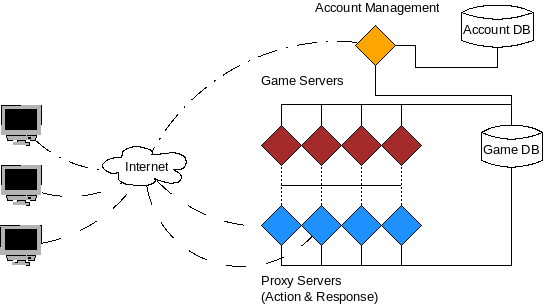
\includegraphics[width=\textwidth]{img/cap2/game_with_proxy.png}
\centering

Adaptado de:~\cite{1417630}.
\end{figure}



A infraestrutura do servidor de jogo contém um \textit{Proxy Server Farm} utilizando o algoritmo \textit{Round Robin} com pesos para balanceamento de carga entre cada cliente.
%
Cada \textit{Proxy Server} é responsável por comunicar com os demais microsserviços privados ao servidor, baseado com a área de interesse de sua conexão.
%
O protocolo de comunicação utilizado entre o Cliente e \textit{Proxy Server} é baseado em \ac{rpc}~\cite{faber, borella}, porém não é relatado sobre o o protocolo de comunicação utilizado entre o \textit{Proxy Server} e o \textit{Game Server}.
%
A sua arquitetura pode ser observada na Figura \ref{fig:game_with_proxy}, na qual obteve seus dados durante 100 dias para realizar as análises.
%
A Figura \ref{fig:players_peer_time} demonstra uma amostra do número de conexões pelo tempo no serviço obtido.



\begin{figure}[htb!]
\caption{Número de conexões no serviço pelo tempo decorrido.}
\label{fig:players_peer_time}
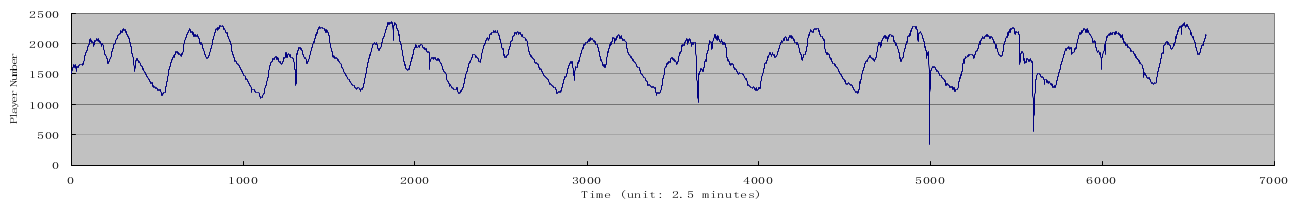
\includegraphics[width=\textwidth]{img/cap2/players_peer_time.png}
\centering

Fonte:~\cite{1417630}.
\end{figure}



Como análise, o autor correlacionou o número de conexões com número de pacotes e banda, consumidos, utilizando uma função estatística linear.
%
Esta função pode ser utilizada com regressão linear para prever consumo de recursos futuros e por fim realocar mais recursos ao serviço, contribuindo com escalabilidade vertical autônoma.
%
Um exemplo de aplicação dessa regressão linear pode ser visualizada na Figura~\ref{fig:regressao_bytes}, no qual o autor compara o consumo de banda real comparado a regressão linear.



\begin{figure}[htb!]
\caption{Regressão linear comparado ao consumo de banda real do servidor.}
\label{fig:regressao_bytes}
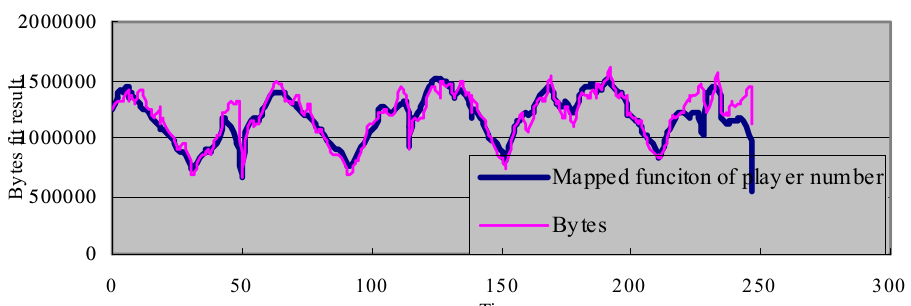
\includegraphics[width=\textwidth]{img/cap2/regressao.png}
\centering

Fonte:~\cite{1417630}
\end{figure}



Entretanto, a escalabilidade horizontal não pode ser prevista, visto que não é analisado o posicionamento de cada personagem a fim de dividir os ambientes em pedaços menores com outros serviços.
%
Como trabalhos futuros é relatado a análise do posicionamento de personagens para escalabilidade horizontal, a análise de outras arquiteturas e a análise de outros gêneros de jogos, além do impacto de utilizar balanço de carga e provisionamento de recursos de forma dinâmica.



\section{Villamizar et al. (2016)}



O trabalho de ~\cite{7515686} investiga o custo de arquiteturas de microsserviços, arquiteturas \ac{paas} orientadas a eventos e aplicações monolíticas para aplicações web.
%
A sua principal motivação é a comparação de custos para a tradução de sistemas legados para arquiteturas distribuídas.
%
Para isso, o autor preparou três instâncias de testes com suas configurações desenhadas a fim de ter o maior número de requisições por minuto com o mesmo custo financeiro.



\begin{figure}[htb!]
\caption{Arquitetura monolítica web implementada na \ac{aws}.}
\label{fig:aws_monolitico}
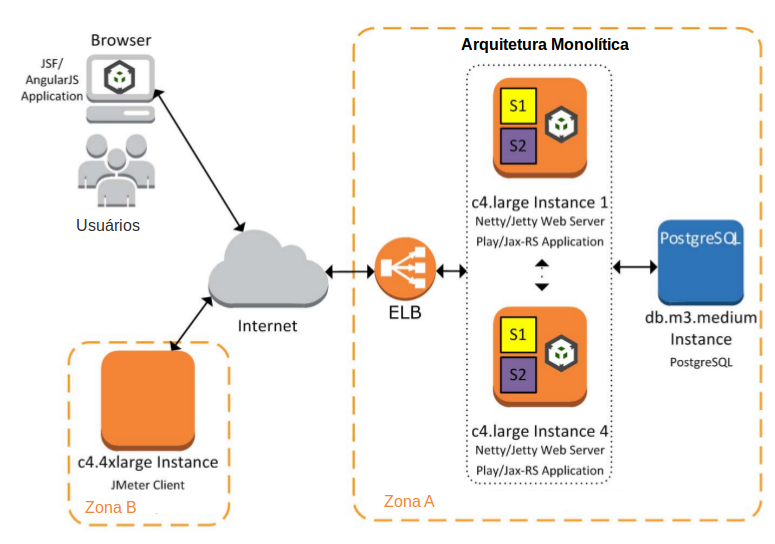
\includegraphics[width=\textwidth]{img/cap2/aws_monolitico.png}
\centering

Fonte:~\cite{7515686}
\end{figure}


\textbf{Instância I.} Utilizando quatro instâncias \ac{aws} \textit{c4.large}, uma instância \ac{aws} \textit{c4.xlarge} e uma instância \ac{aws} \textit{db.m3.medium}.
%
A Figura~\ref{fig:aws_monolitico} exibe a implantação de uma aplicação web monolítica.
%
Essa arquitetura foi implementada utilizando \textit{Jax-RS} e \textit{Play Framework}.




\begin{figure}[htb!]
\caption{Arquitetura de microsserviços web implementada na \ac{aws}.}
\label{fig:aws_microsservicos}
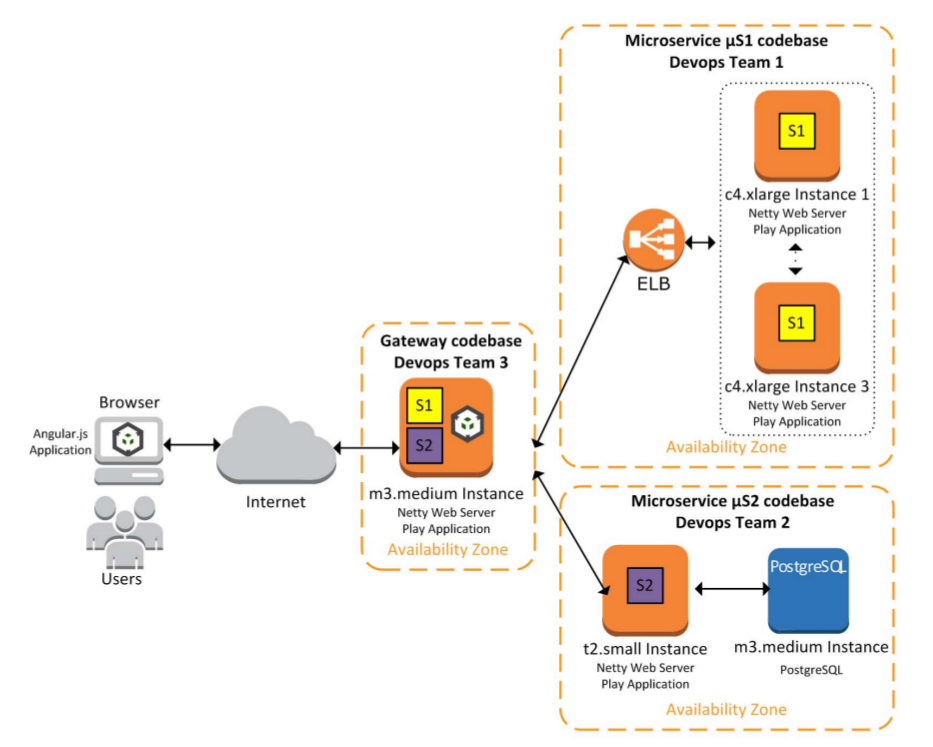
\includegraphics[width=\textwidth]{img/cap2/aws_microsservicos.png}
\centering

Fonte:~\cite{7515686}
\end{figure}

\textbf{Instância II.} Utilizando três instâncias \ac{aws} \textit{c4.xlarge}, uma instância \ac{aws} \textit{t2.small} e uma instância \ac{aws} \textit{db.m3.medium}.
%
A Figura~\ref{fig:aws_microsservicos} exibe a implantação de uma aplicação de microsserviços web. Essa arquitetura foi implementada utilizando \textit{Play Framework}, framework para desenvolvimento web para a linguagem Java e Scala~\footnote{Play Framework: \url{https://www.playframework.com/}}.



\begin{figure}[htb!]
\caption{Arquitetura de microsserviços web implementada na \ac{aws} utilizando a tecnologia \textit{lambda}.}
\label{fig:aws_lambda}
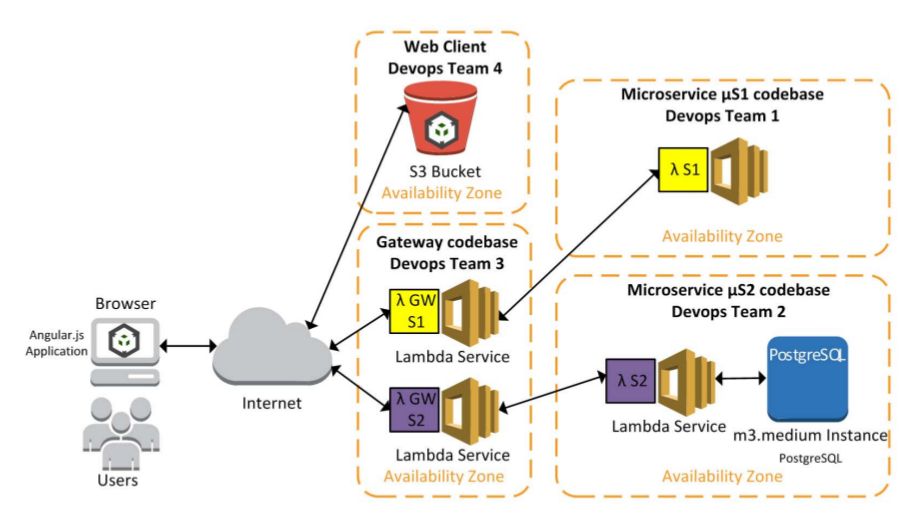
\includegraphics[width=\textwidth]{img/cap2/aws_lambda.png}
\centering

Fonte:~\cite{7515686}
\end{figure}

\textbf{Instância III.} Utilizando duas instâncias \ac{aws} \textit{lambda S1}, duas instâncias \ac{aws} \textit{lambda S2}, uma instância \ac{aws} \textit{S3 Bucket} e uma instância \ac{aws} \textit{db.m3.medium}.
%
A Figura~\ref{fig:aws_lambda} exibe a implantação de uma aplicação de microsserviços web utilizando a tecnologia \ac{aws} \textit{lambda}. Essa arquitetura foi implementada utilizando o \textit{framework} \textit{Node.js}\footnote{Node.js: \url{https://nodejs.org/en/}}, nas quais as funções de \textit{gateway} são implementadas em quatro funções independentes do tipo \textit{microservice-http-endpoint}.



\begin{figure}[htb!]
\caption{Custo por um milhão de requisições em dólares utilizando diferentes arquiteturas sobre a \ac{aws}.}
\label{fig:custo_aws}
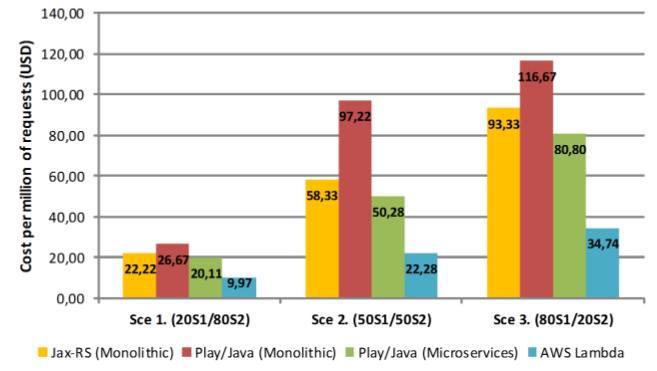
\includegraphics[width=\textwidth]{img/cap2/custo_aws.png}
\centering

Fonte:~\cite{7515686}
\end{figure}



Foi concluído que a arquitetura de microsserviços, nas condições desta aplicação, podem reduzir até 13.42\% em gastos com a infraestrutura.
%
Essa redução pode ser observada na Figura~\ref{fig:custo_aws}.
%
O autor alerta sobre tolerância a falhas, transações distribuídas, distribuição de dados e versionamento de serviço.


\section{Suznjevic e Matijasevic (2012)}



O trabalho de ~\cite{6374456} tem seu objetivo a fim de prever a carga a qual um serviço \ac{mmorpg} pode receber utilizando a complexidade das operações nos contextos de \ac{pvp} e \ac{pvnpc} a qual um personagem pode realizar em um ambiente.
%
Este trabalho usa com base o modelo descrito na Seção~\ref{sec:huang}, um modelo distribuído em serviços na qual efetuam o processamento de uma região do ambiente virtual.



\begin{table}[htb!]
\centering
\caption{Complexidade da interação com o ambiente, por contexto da interação.}
\label{tab:complexidade}
\begin{tabular}{|l|l|l|l|l|}
\hline
Contexto da ação        & \ac{pvp}           & \ac{pvnpc}              & Número de \acp{npc}    & Network {[}kbits/s{]} \\ \hline
Questing                & $O(n)$             & $O(n log(n))$           & $N \leq 6 $            & 11.4          \\ \hline
Trading                 & $O(n)$             & $O(n)$                  & $N \leq 20$            & 8.1           \\ \hline
Dungeons                & $O(n^2)$           & $O(n^2)$                & $N \leq 20$            & 18.3          \\ \hline
\ac{pvp} combat         & $O(n^3)$           & $O(n)$                  & $N = 0    $            & 24.1          \\ \hline
Raiding                 & $O(n^2 log(n))$    & $O(n^3)$                & $N \leq 40$            & 32.0          \\ \hline
\end{tabular}

Fonte:~\cite{6374456}
\end{table}


A análise realizada leva em conta a complexidade das ações no ambiente, a qual pode ser descrita na Tabela~\ref{tab:complexidade}.
%
Essa tabela exibe as ações que podem ser executadas para interagir com o ambiente, seja essa interação com \ac{pvp} (jogador com outro jogador) ou \ac{pvnpc} (jogador com um personagem ou objeto gerenciado pelo serviço).
%
Os contextos analisados nessa tabela são:

\begin{itemize}
  \item \textit{Questing}: Contexto de missão, na qual um grupo de jogadores ou um grupo de \acp{npc} podem ser afetados nas ações.
  \item \textit{Trading}: Contexto de negociação, na qual a complexidade leva em conta somente o número de itens negociados.
  \item \textit{Dungeons}: Contexto de exploração, na qual o ambiente pode ser modificado conforme as ações dos personagens em um ambiente isolado para este grupo.
  \item \textit{\ac{pvp} combat}: Contexto de batalha entre jogadores, na qual as ações entre os jogadores influenciam diretamente o estado do personagem oponente.
  \item \textit{Raiding}: Representa um contexto específico de exploração, na qual múltiplos jogadores unem forças a fim de combater outro grupo de jogadores ou \acp{npc}.
\end{itemize}


\begin{figure}[htb!]
\caption{Regressão levando em conta a complexidade das ações e contexto dos personagens.}
\label{fig:regressao_complexidade}
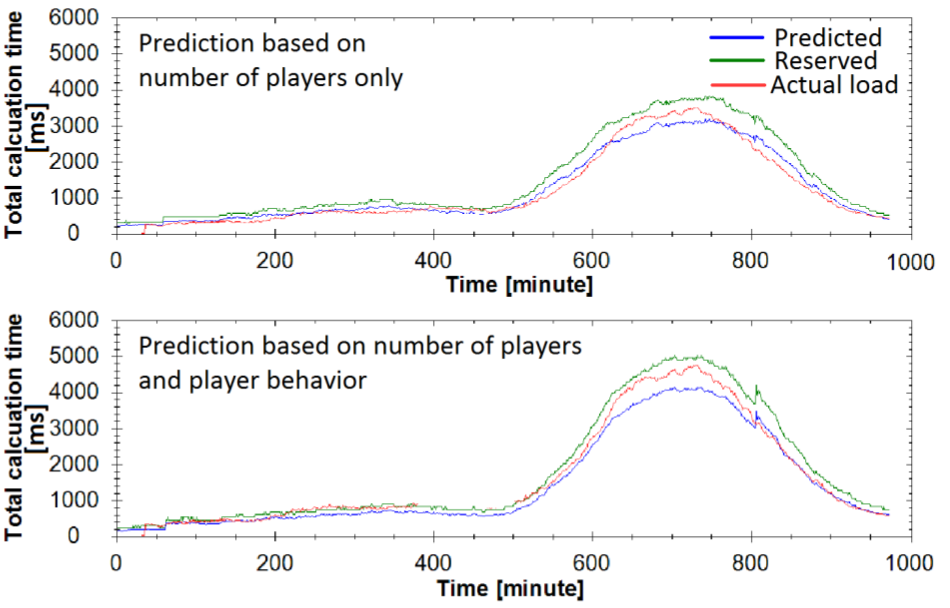
\includegraphics[width=\textwidth]{img/cap2/network_regressao_complexidade.png}
\centering

Fonte:~\cite{6374456}
\end{figure}


A abordagem utilizou as complexidades das ações, o número de conexões e o contexto de cada personagem no ambiente para predizer a banda utilizada.
%
Pode-se visualizar uma regressão na Figura~\ref{fig:regressao_complexidade}.



O autor conclui que o contexto de interação com o ambiente de cada personagem tem relevância com o consumo de \ac{cpu} e banda, a qual pode ser calculada com sua complexidade a fim de desenvolver uma ferramenta para predição de carga sobre serviços \ac{mmorpg}.
%
Entretanto, essa predição não é feita em tempo real, não contribuindo para a automação da escalabilidade vertical e horizontal da arquitetura de microsserviços.



\section{Análise dos trabalhos relacionados}
\label{sec:similares_analise}



Para os trabalhos relacionados, são analisados o tipo de pesquisa realizado sobre Microsserviços e serviços \ac{mmorpg}.
%
Também são levantados quais os recursos computacionais relacionados com estas análises.


Nos trabalhos relacionados existem duas abordagens utilizadas pelos autores, na qual estão relacionados a Previsão de Carga ou Comparação entre Arquiteturas de microsserviços~\cite{7515686, 6374456}:

\begin{itemize}
  \item \textbf{Comparação de arquiteturas}: O autor utiliza alguma métrica a fim de decidir qual a melhor alternativa de arquitetura para determinada aplicação.
  \item \textbf{Previsão de carga}: Projetar a carga futura sobre algum recurso a fim de escalar automaticamente a sua arquitetura na nuvem, a fim de reduzir gastos de recursos ociosos e diminuir o impacto de ocorrências aos usuários finais.
\end{itemize}

Dessa forma, pode-se dividir os trabalhos relacionados com a sua categoria.
%
Esta relação pode ser visualizada na Tabela~\ref{tab:categoria_trabalhos}.

\begin{table}[htb!]
\centering
\caption{Trabalhos relacionados por categoria.}
\label{tab:categoria_trabalhos}
\begin{tabular}{l|l}
\hline
Autor & Categoria                            \\ \hline
\cite{6374456}  & Previsão de carga          \\ \hline
\cite{7515686}  & Comparação de arquiteturas \\ \hline
\cite{1417630}  & Previsão de carga          \\ \hline
\end{tabular}


Fonte: O próprio autor.
\end{table}

Para o trabalho referente a comparação de arquiteturas~\cite{7515686}, o recurso utilizado foi o custo por um determinado número de requisições web.
%
Já para os trabalhos referentes a previsão de carga~\cite{6374456, 1417630} foi levantado o consumo da banda, \ac{cpu} e memória, entretanto não levantou-se o número de conexões e latência aos usuários, na qual podem ser observados na Tabela~\ref{tab:recursos_categoria}.
%
Nenhum trabalho relatou limite de conexões ou latência do sistema.

\begin{table}[htb!]
\centering
\begin{adjustbox}{max width=\textwidth}
\caption{Trabalhos relacionados por recurso analisado.}
\label{tab:recursos_categoria}
\begin{tabular}{l|l|l|l|l|l|l|l}
\hline
Autor           & \ac{cpu}   & Memória    & Banda      & Custo      & Latência & \makecell{Limite \\ de \\ conexões} & \makecell{Complexidade \\ de \\ Algoritmos} \\ \hline
\cite{1417630}  & $\times$   & $\times$   & \checkmark & $\times$   & $\times$ & $\times$                            & $\times$                                    \\ \hline
\cite{7515686}  & $\times$   & $\times$   & $\times$   & \checkmark & $\times$ & $\times$                            & $\times$                                    \\ \hline
\cite{6374456}  & \checkmark & \checkmark & \checkmark & $\times$   & $\times$ & $\times$                            & \checkmark                                  \\ \hline
\end{tabular}
\end{adjustbox}

Fonte: O próprio autor.
\end{table}



Outro ponto a ser analisado são as arquiteturas utilizadas. Os trabalhos referentes a previsão de carga não utilizaram uma arquitetura de microsserviços, mesmo sendo um sistema distribuído.
%
Nesses serviços, os sistemas eram dependentes entre sí e precisavam um dos outros para o seu funcionamento.
%
A relação de arquiteturas abordadas pode ser visualizado na Tabela~\ref{tab:arquiteturas_analisadas}, na qual mostra quais trabalhos abordaram os temas sobre arquiteturas de microsserviços e jogos \ac{mmorpg}.
%
Além disso, não foi descrito um método de replicação automática dos serviços a fim de prover alta disponibilidade de forma automatizada, sendo abordado como um trabalho futuro.


\begin{table}[htb!]
\centering
\begin{adjustbox}{max width=\textwidth}
\caption{Arquiteturas analisadas.}
\label{tab:arquiteturas_analisadas}
\begin{tabular}{l|l|l|l}
\hline
Autor           & Arquitetura de Microsserviços & Arquitetura Distribuída  & \ac{mmorpg}   \\ \hline
\cite{1417630}  & $\times$                      & \checkmark               & \checkmark    \\ \hline
\cite{7515686}  & \checkmark                    & \checkmark               & $\times$      \\ \hline
\cite{6374456}  & $\times$                      & \checkmark               & \checkmark    \\ \hline
\end{tabular}
\end{adjustbox}

Fonte: O próprio autor.
\end{table}


Este Trabalho de Conclusão de Curso pretende analisar uma arquitetura de microsserviços especificada a jogos \ac{mmorpg}, visando métricas de desempenho e custo de operação.
%
Os recursos analisados serão CPU, Memória, Banda, Custo, Latência, Limite de Conexões e Complexidade dos Algoritmos empregados.


\section{Considerações parciais}

Após a busca de trabalhos relacionados, encontrou-se três principais trabalhos a qual analisam ora arquiteturas de microsserviços ora arquiteturas de jogos \ac{mmorpg}.
%
Nesse sentido, tais trabalhos relacionados não realizam uma intercessão entre ambos os temas, a qual o atual trabalho propõe a análise.
%
Também foi identificado as métricas a qual estes trabalhos analisaram.
%
Nesse sentido, o atual trabalho irá propor a análise sobre as mesmas métricas, entretanto completando com métricas que são de interesse para analisar pontos de falha em tais arquiteturas.

Por fim, foi apresentado trabalhos relacionados a qual guiaram os moldes do plano de testes e a proposta deste trabalho, porém com utilizando ambos os temas de arquiteturas de microsserviços e jogos \ac{mmorpg}, realizando uma análise com mais características sobre o serviço do jogo.
